%!TEX root = ../main.tex

% show warning for old LaTeX syntax
\RequirePackage[l2tabu, orthodox]{nag}

\usepackage{xstring}
\usepackage[utf8]{inputenc}
\usepackage[T1]{fontenc}

% iflang command definition
\newcommand{\iflang}[2]{%
    \IfStrEq{\documentLanguage}{#1}{#2}{}%
}

% ifDocType comand definition
\newcommand{\ifDocType}[3]{%
    \IfStrEq{\documentType}{#1}{#2}{#3}%
}

% ifMultipleAuthors definition
\newcommand{\ifMultipleAuthors}[2]{%
    \IfStrEq{\multipleAuthors}{true}{#1}{#2}%
}

% ifSpecialDocument definition
\newcommand{\ifSpecialDocument}[2]{\IfStrEqCase{\documentType}{%
        {T3\_1000}{#2\ignorespaces}%
        {T3\_2000}{#2\ignorespaces}%
        {T3\_3100}{#2\ignorespaces}%
        {T3\_3300}{#2\ignorespaces}%
}[#1\ignorespaces]%
}

% Include main settings
%!TEX root = ./main.tex

%%**************************************************************
%%
%% DHBW Heidenheim - Template for Bachelor Thesis
%%
%% Bevor usisng this template please have a look at the REAMDME.md file
%%
%%**************************************************************

\documentclass[
    pdftex,
    oneside,
    12pt,                   % fontsize
    parskip=half,           % Space (in lines) between paragraphs
    headheight = 12pt,      % Header hight
    headsepline,            % Line after header
    footheight = 16pt,      % Footer height
    footsepline,            % Line before footer
    abstracton=true,        % Abstract headline
    DIV=calc,               % Calculate print space
    BCOR=8mm,               % BCOR settings (Bindekorrektur)
    headinclude=false,      % Exclude header from print space
    footinclude=false,      % Exclude footer from print space
    listof=totoc,           % Show List of Figures/Tables in Contents
    toc=bibliography,       % Show Bibliography in Contents
]{scrreprt}

%!TEX root = ../main.tex

% show warning for old LaTeX syntax
\RequirePackage[l2tabu, orthodox]{nag}

\usepackage{xstring}
\usepackage[utf8]{inputenc}
\usepackage[T1]{fontenc}

% iflang command definition
\newcommand{\iflang}[2]{%
    \IfStrEq{\documentLanguage}{#1}{#2}{}%
}

% ifDocType comand definition
\newcommand{\ifDocType}[3]{%
    \IfStrEq{\documentType}{#1}{#2}{#3}%
}

% ifMultipleAuthors definition
\newcommand{\ifMultipleAuthors}[2]{%
    \IfStrEq{\multipleAuthors}{true}{#1}{#2}%
}

% ifSpecialDocument definition
\newcommand{\ifSpecialDocument}[2]{\IfStrEqCase{\documentType}{%
        {T3\_1000}{#2\ignorespaces}%
        {T3\_2000}{#2\ignorespaces}%
        {T3\_3100}{#2\ignorespaces}%
        {T3\_3300}{#2\ignorespaces}%
}[#1\ignorespaces]%
}

% Include main settings
%!TEX root = ./main.tex

%%**************************************************************
%%
%% DHBW Heidenheim - Template for Bachelor Thesis
%%
%% Bevor usisng this template please have a look at the REAMDME.md file
%%
%%**************************************************************

\documentclass[
    pdftex,
    oneside,
    12pt,                   % fontsize
    parskip=half,           % Space (in lines) between paragraphs
    headheight = 12pt,      % Header hight
    headsepline,            % Line after header
    footheight = 16pt,      % Footer height
    footsepline,            % Line before footer
    abstracton=true,        % Abstract headline
    DIV=calc,               % Calculate print space
    BCOR=8mm,               % BCOR settings (Bindekorrektur)
    headinclude=false,      % Exclude header from print space
    footinclude=false,      % Exclude footer from print space
    listof=totoc,           % Show List of Figures/Tables in Contents
    toc=bibliography,       % Show Bibliography in Contents
]{scrreprt}

\input{ads/header}

\input{content/glossary}

\begin{document}

    % Cover
    \begin{spacing}{1}
        \input{ads/cover}
    \end{spacing}
    \newpage

    \pagenumbering{Roman}

    % Restriction notices
    %    \input{ads/restrictionNotices}
    %    \newpage


    % Declaration
    \input{ads/declaration}
    \newpage

    % Abstract
    %\input{content/abstract}
    %\newpage

    % only page number in footer
    \pagestyle{plain}

    % space bevore chapter headline
    \RedeclareSectionCommand[beforeskip=\chapterMargin]{chapter}

    % Contents
    \begin{spacing}{1.1}
        \begingroup

        % set subchapter depth
        \setcounter{tocdepth}{2}

        \tableofcontents
        \clearpage
        \endgroup
    \end{spacing}
    \newpage

    % Acronyms
    \cleardoublepage
    \input{content/acronyms}

    % List of Figures
    \cleardoublepage
    \listoffigures

    %List of Tables
    % \cleardoublepage
    % \listoftables

    % List of Listings
    \cleardoublepage
    \lstlistoflistings
    \cleardoublepage

    \pagenumbering{arabic}

    \pagestyle{headings}

    %Content
    \foreach \i in {01,02,03,04,05,06,07,08,09,...,99} {%
        \edef\FileName{content/chapter/\i .tex}%
        \IfFileExists{\FileName}{%
            \input{\FileName}}
    }

    \clearpage

    % Bibilography
    \cleardoublepage
    \printbibliography[heading=bibintoc,title={Literaturverzeichnis}]

    % Glossar
    % \cleardoublepage
    % \printglossary[style=altlist,title=\glossaryPhrase]
    % \input{content/glossary}

    % Appendix
    \clearpage
    \appendix
    \input{content/appendix}

\end{document}


% Include document settings
%!TEX root = ../main.tex

%% Document language (en, de)
\newcommand{\documentLanguage}{de}

%% Document type
% T3\_1000 Project Thesis (Semester 1 & 2)
% T3\_2000 Project Thesis (Semester 3 & 4)
% T3\_3100 Seminar Paper (Semester 5 & 6)
% T3\_3300 Bachelor Thesis
\newcommand{\documentType}{T3\_XXXX}

\newcommand{\multipleAuthors}{false}
\newcommand{\documentAuthor}{Vivian Berger}
\newcommand{\documentTitle}{Titel der Arbeit}
\newcommand{\documentPeriod}{X Wochen}

\newcommand{\matriculationNumber}{9549720}

\newcommand{\locationUniversity}{Heidenheim}
\newcommand{\department}{Informatik}
\newcommand{\course}{HDH-TINF2022}

\newcommand{\degree}{Bachelor of Science}
% INF2014 - INF2016 (MI):       Bachelor of Science
% INF2014 - INF2016 (IA/IM) :   Bachelor of Engineering
% INF2017 (all):                Bachelor of Science

% A lecture that the document is written for
\newcommand{\lecture}{Software Engineering}
% Whether to show the lecture on cover
\newcommand{\showLecture}{false}

\newcommand{\releaseDate}{XX.XX.20XX}
\newcommand{\releaseLocation}{Ulm}

\newcommand{\companyName}{Mercedes-Benz Tech Innovation GmbH}
\newcommand{\companyLocation}{Ulm}

\newcommand{\tutor}{Elmar Schug}
\newcommand{\evaluator}{2. Gutachter}

\newcommand{\linkColor}{0000AF}


% Load language specific Strings
\input{lang/\documentLanguage}

% Load language specific babel package
\iflang{de}{\usepackage[ngerman, english]{babel}}
\iflang{en}{\usepackage[english, ngerman]{babel}}

% Add comment feature
\newcommand{\comment}[1]{\par {\bfseries \color{blue} #1 \par}}


%%%%%%% Package Includes %%%%%%%
\usepackage[margin=\margin,foot=1cm]{geometry}
\usepackage[activate]{microtype}
\usepackage[onehalfspacing]{setspace}
\usepackage{makeidx}
\usepackage[autostyle=true,german=quotes]{csquotes}
\usepackage{longtable}
\usepackage{enumitem}
\usepackage{graphicx}
\usepackage{pdfpages}
\usepackage{xcolor}
\usepackage{float}
\usepackage{array}
\usepackage{calc}
\usepackage[right]{eurosym}
\usepackage{wrapfig}
\usepackage{pgffor}
\usepackage[perpage, hang, multiple, stable]{footmisc}
\usepackage[printonlyused]{acronym}
\usepackage{listings}
\lstset{literate=%
        {Ö}{{\"O}}1
        {Ä}{{\"A}}1
        {Ü}{{\"U}}1
        {ß}{{\ss}}1
        {ü}{{\"u}}1
        {ä}{{\"a}}1
        {ö}{{\"o}}1
        {~}{{\textasciitilde}}1
} % Umlaute in Listings
\usepackage[obeyFinal,backgroundcolor=yellow,linecolor=black]{todonotes}
\usepackage{rotating}
\usepackage{lscape}
\usepackage{amsmath}
\usepackage{amssymb}
\usepackage{\documentFont}
\usepackage[%
    breaklinks,
    pdftitle={\documentTitle},
    pdfauthor={\documentAuthor},
    pdfsubject={\documentType},
    pdfcreator={pdflatex, LaTeX with KOMA-Script},
    pdfpagemode=UseOutlines,     % Show Contents while opening
    pdfdisplaydoctitle=true,     % Show document title instead of file name
    pdflang={\documentLanguage}, % Document language
]{hyperref}
\usepackage{bookmark}
\usepackage[nonumberlist,toc]{glossaries}
\usepackage{amsfonts}
\usepackage{pgfplots}
\usepackage{placeins}
\pgfplotsset{compat=1.15}
\usepackage{mathrsfs}
\usetikzlibrary{arrows}

\usepackage{circledsteps}

% %!TEX root = ../main.tex

%%%%%%% Code Highlighting with minted and pygements %%%%%%%%
% Python and Python Package Pygments needed
% docs: https://ctan.kako-dev.de/macros/latex/contrib/minted/minted.pdf

%%%%%%%%%%%%%%%%%%%%%%%%%%%%%%%%%%%%%%%%%%%%%%%%%%%%%%%%%%%%
%%              See documentation at line 65              %%
%%%%%%%%%%%%%%%%%%%%%%%%%%%%%%%%%%%%%%%%%%%%%%%%%%%%%%%%%%%%

\usepackage{keyval}
\usepackage{kvoptions}
\usepackage{fancyvrb}
\usepackage{fvextra}
\usepackage{upquote}
\usepackage{ifthen}
\usepackage{ifplatform}
\usepackage{pdftexcmds}
\usepackage{etoolbox}
\usepackage{lineno}
\usepackage{caption}
\usepackage{catchfile}
\usepackage[many]{tcolorbox}
\usepackage[outputdir=../out]{minted}
\tcbuselibrary{minted}

% make fcolorbox a dummy for code blocks so that the red boxes for syntax errors are disabled
\AtBeginEnvironment{code}{%
    \renewcommand{\fcolorbox}[4][]{#4}}

%%                                                 v  change emacs to change the default style
\AtBeginDocument{%
    \newtcblisting[blend into=listings]{code}[4][emacs]{
        title={#3},
        phantomlabel=#4,
        listing engine=minted,
        minted language=#2,
        minted style=#1,
        minted options={
            linenos,
            autogobble,
            breaklines,
            breakbefore={.|&!+-*/},
            breakafter={,:()\{\}\space},
            fontsize=\footnotesize,
            xleftmargin=0.2em,
            numbers=left,
            numbersep=1em,
            baselinestretch=1,
            escapeinside=°°
        },
        listing only,
        breakable,
        enhanced jigsaw,
        colframe=black,
        sharp corners,
        boxrule=2pt,
        colback=white,
        left=0em,
        left skip=1.5em,
        width=\linewidth-1.5em
    }
}

% workaround for custom syntax highlighting
% you must escape this inside the code block with semicolons
\definecolor{greenForTypes}{rgb}{0, 0.5, 0}
\newcommand{\typeName}[1]{\textbf{\textcolor{greenForTypes}{#1}}}
% example:
% \begin{code}{react}{Title}{lst:ReactComponent}
%     export default function Component(props: ;\typeName{ComponentProps};) {
% ...

% check available styles with:
%   pygmentize -L styles
% in the terminal

% check available languages with:
%   pygmentize -L lexers
% in the terminal

% use the environment like this:
% \begin{code}{LANGUAGE}{CAPTION}{LABEL}
%   <the actual code>
% \end{code}

% or if you want to specify the style, use the environment like this:
% \begin{code}[STYLE]{LANGUAGE}{CAPTION}{LABEL}
%   <the actual code>
% \end{code}

% You can change the default style in line 29 by replacing the text in the last [] to the desired default style

% for example:
% \begin{code}{python}{Python Code}{lst:PythonCode}
% def fibonacci(n):
%   x = 0
%   y = 1
%   for i in range(n):
%       x, y = y, x + y
%   return x
%
% if __name__ == "__main__":
%   import sys
%
%   n = int(sys.argv[1])
%   print(fibonacci(10))
% \end{code}

\usepackage[export]{adjustbox}
\usepackage{booktabs}
\usepackage{abstract}
\usepackage{lipsum}

% Generate glossary
\makeglossaries{}

% Load colors
\defineColors{}

% Set Titel, Autor and Date
\title{\documentTitle}
\author{\documentAuthor}
\date{\datum}


% PDF link settings
\hypersetup{%
    colorlinks=true,
    linkcolor=LinkColor,
    citecolor=LinkColor,
    filecolor=LinkColor,
    menucolor=LinkColor,
    urlcolor=LinkColor,
    linktocpage=true,
    bookmarksnumbered=true
}

% Captions fontsize
\addtokomafont{caption}{\small}

% Bibliographie settings
\iflang{de}{%
    \usepackage[
        backend=biber,        % recommended. Alternative: bibtex
        bibwarn=true,
        bibencoding=utf8,             % If .bib file is encoded with utf8, otherwise ascii
        sortlocale=de_DE,
        style=\quoteStyle,
    ]{biblatex}
}
\iflang{en}{%
    \usepackage[
        backend=biber,        % recommended. Alternative: bibtex
        bibwarn=true,
        bibencoding=utf8,        % If .bib file is encoded with utf8, otherwise ascii
        sortlocale=en_US,
        style=\quoteStyle,
    ]{biblatex}
}

% break long links in bibliography
\setcounter{biburllcpenalty}{7000}
\setcounter{biburlucpenalty}{8000}

\addbibresource{bibliography.bib}

% Hurenkinder und Schusterjungen verhindern
% http://projekte.dante.de/DanteFAQ/Silbentrennung
\clubpenalty = 10000 % schließt Schusterjungen aus (Seitenumbruch nach der ersten Zeile eines neuen Absatzes)
\widowpenalty = 10000 % schließt Hurenkinder aus (die letzte Zeile eines Absatzes steht auf einer neuen Seite)
\displaywidowpenalty=10000

% Graphicspath
\graphicspath{{images/}}


% "define" Scala
\lstdefinelanguage{Scala}{
    morekeywords={abstract,case,catch,class,def,%
    do,else,extends,false,final,finally,%
    for,if,implicit,import,match,mixin,%
    new,null,object,override,package,%
    private,protected,requires,return,sealed,%
    super,this,throw,trait,true,try,%
    type,val,var,while,with,yield},
    keywordstyle=\color{blue},
    otherkeywords={\%,\<,\>,\#,\$},
    sensitive=true,
    morecomment=[l]{//},
    morecomment=[n]{/*}{*/},
    morestring=[b]",
    morestring=[b]',
    morestring=[b]""",
    ndkeywords={@Deprecated, @JvmField, @JvmName, @JvmOverloads, @JvmStatic, @JvmSynthetic, @RunWith, Array, DoubleArray, FloatArray, Byte, Double, Float, Int, Integer, Iterable, Long, Runnable, Short, String, Unit},
    ndkeywordstyle={\color{orange}\bfseries},
}

%\lstset{frame=tb,
%    language=Scala,
%    aboveskip=3mm,
%    belowskip=3mm,
%    showstringspaces=false,
%    columns=flexible,
%    basicstyle={\small\ttfamily},
%    numbers=none,
%    numberstyle=\tiny\color{gray},
%    frame=single,
%    breaklines=true,
%    breakatwhitespace=true,
%    tabsize=3,
%    stringstyle=\color[rgb]{0.0,0.55,0.0}
%}

\lstdefinelanguage{Kotlin}{
    comment=[l]{//},
    emphstyle={\color{red}},
    identifierstyle=\color{black},
    morekeywords=[2]{},
    morekeywords=[3]{},
    keywordstyle=[2]\color{red},
    keywordstyle=[3]\color[rgb]{0.0,0.0,0.75},
    keywords={!in, !is, abstract, actual, annotation, as, as?, break, by, catch, class, companion, const, constructor, continue, crossinline, data, delegate, do, dynamic, else, enum, expect, external, false, field, file, final, finally, for, fun, if, import, in, infix, init, inline, inner, interface, internal, is, lateinit, noinline, null, object, open, operator, out, override, package, param, private, property, protected, public, receiveris, reified, return, return@, sealed, set, setparam, super, suspend, tailrec, this, throw, true, try, typealias, typeof, val, var, vararg, when, where, while},
    morecomment=[s]{/*}{*/},
    morestring=[b]",
    morestring=[s]{"""*}{*"""},
    ndkeywords={@Deprecated, @JvmField, @JvmName, @JvmOverloads, @JvmStatic, @JvmSynthetic, Array, DoubleArray, FloatArray, Byte, Double, Float, Int, Integer, Iterable, Long, Runnable, Short, String, Unit},
    ndkeywordstyle={\color{orange}\bfseries},
    sensitive=true,
    showstringspaces=false,
    keywordstyle=\color[rgb]{0.9,0.1,0.9},
    commentstyle=\color[rgb]{0.6,0.6,0.6}
}
\definecolor{dkgreen}[rgb]{0.0,0.55,0.0}

% frequently used programing languages
\lstloadlanguages{PHP,Python,Java,Kotlin,C,C++,bash}

\listingsettings{}
% Rename Listings
\renewcommand\lstlistingname{\listingPhrase}
\renewcommand\lstlistlistingname{\listListingPhrase}
\def\lstlistingautorefname{\authorListingPhrase}

% Spaces in tables
\setlength{\tabcolsep}{\tableColumnMargin}
\renewcommand{\arraystretch}{\tableRowMargin}


%!TEX root = ../main.tex

%
% To create glossary run the following command: 
% makeglossaries main.acn && makeglossaries main.glo
%

%
% Glossareintraege --> referenz, name, beschreibung
% Aufruf mit \gls{...}
%


\begin{document}

    % Cover
    \begin{spacing}{1}
        %!TEX root = ../main.tex

\begin{titlepage}
	\begin{longtable}{p{4cm} p{11cm}}
		\raggedright {\raisebox{\ht\strutbox-\totalheight}{
\includegraphics[width=5cm]{images/cover/logo-dhbw}}} &
		\ifDocType{T3\_3100}{}{
			\ifSpecialDocument{}{%
				\raggedleft {\raisebox{\ht\strutbox-\totalheight}{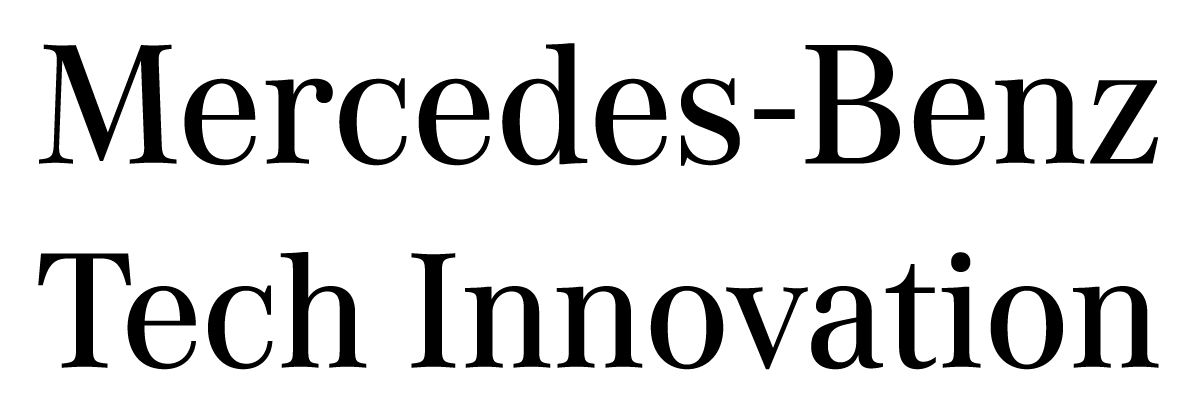
\includegraphics[width=7cm]{images/cover/company-logo}}}
			}%
		}
	\end{longtable}
	\enlargethispage{20mm}
	\begin{center}
		\doublespacing{
		\vspace*{12mm}	{\LARGE\textbf \documentTitle }}\\
		\vspace*{12mm}	{\large\textbf {\documentTypePhrase}}\\
		
		% degre only for bachelor thesis
		\ifDocType{T3\_3300}{
			\vspace*{12mm}	\degreePhrase\\
			\vspace*{3mm}		{\textbf \degree}\\
		}

		\IfStrEq{\showLecture}{true}{
			\vspace*{12mm}	\lecturePhrase\\
			\vspace*{0mm}		{\textbf \lecture}\\
		}

		\vspace*{12mm}	\departmentPhrase{} \department\\
    \vspace*{0mm}		\locationUniversityPhrase{} \locationUniversity\\
		\vspace*{12mm}	\documentAuthorPhrase\\
		\vspace*{3mm}		{\large\textbf \documentAuthor}\\
		\vspace*{12mm}	\releaseDate\\
	\end{center}
	\vfill
	\begin{spacing}{1.2}
	\begin{tabbing}
		mmmmmmmmmmmmmmmmmmmmmm             \= \kill
		\textbf{\documentPeriodPhrase}       \>  \documentPeriod\\
		\textbf{\matriculationNumberPhrase, \coursePhrase}  \>  \matriculationNumber, \course\\

		% no company for the semester paper and special documents
		\ifDocType{T3\_3100}{}{%
			\ifSpecialDocument{}{%
				\textbf{\companyPhrase}                  \>  \companyName, \companyLocation\\
			}%
		}%
		\textbf{\tutorPhrase}               \>  \tutor\\

		% evaluator only for bachelor thesis
		\ifDocType{T3\_3300}{%
			\textbf{\evaluatorPhrase}              \>  \evaluator
		}{}
	\end{tabbing}
	\end{spacing}
\end{titlepage}

    \end{spacing}
    \newpage

    \pagenumbering{Roman}

    % Restriction notices
    %    %!TEX root = ../main.tex

\thispagestyle{empty}

\section*{\restrictionNoticesPhrase}

\vspace*{2em}

\iflang{de}{%
  Die vorliegende {\documentTypePhrase} mit dem Titel {\itshape{} \documentTitle{}\/} enthält 
  unternehmensinterne bzw. vertrauliche Informationen der {\companyName}, ist deshalb mit einem 
  Sperrvermerk versehen und wird ausschließlich zu Prüfungszwecken am Studiengang {\department} 
  der Dualen Hochschule Baden-Württemberg {\locationUniversity} vorgelegt. Sie ist ausschließlich zur 
  Einsicht durch den zugeteilten Gutachter, die Leitung des Studiengangs und ggf. den Prüfungsausschuss 
  des Studiengangs bestimmt. Es ist untersagt,
  \begin{itemize}
  \item den Inhalt dieser Arbeit (einschließlich Daten, Abbildungen, Tabellen, Zeichnungen usw.) als 
            Ganzes oder auszugsweise weiterzugeben,
  \item Kopien oder Abschriften dieser Arbeit (einschließlich Daten, Abbildungen, Tabellen, 
             Zeichnungen usw.) als Ganzes oder in Auszügen anzufertigen,
  \item diese Arbeit zu veröffentlichen bzw. digital, elektronisch oder virtuell zur Verfügung zu stellen. 
  \end{itemize}
Jede anderweitige Einsichtnahme und Veröffentlichung – auch von Teilen der Arbeit – bedarf der 
vorherigen Zustimmung durch den Verfasser und der {\companyName}.
}

%http://www.ib.dhbw-mannheim.de/fileadmin/ms/bwl-ib/Downloads_alt/Leitfaden_31.05.pdf

\iflang{en}{%
  The {\documentTypePhrase} on hand
  \begin{center}{\itshape{} \documentTitle{}\/}\end{center}
   contains internal resp.\ confidential data of {\companyName}. It is intended solely for inspection by the
   assigned examiner, the head of the {\department} department and, if necessary, the Audit
   Committee \locationUniversityPhrase{} {\locationUniversity}. It is strictly forbidden
    \begin{itemize}
    \item to distribute the content of this paper (including data, figures, tables, charts etc.) as a whole or 
              in extracts,
    \item to make copies or transcripts of this paper or of parts of it,
    \item to display this paper or make it available in digital, electronic or virtual form.
    \end{itemize}
  Exceptional cases may be considered through permission granted in written form by the author 
  and {\companyName}.
}

\vspace{3em}

\releaseLocation, \releaseDate
\vspace{4em}

\rule{6cm}{0.4pt}\\
\documentAuthor

    %    \newpage


    % Declaration
    %!TEX root = ../main.tex

\thispagestyle{empty}

\section*{\declarationPhrase}

\vspace*{2em}

\iflang{de}{%
  \ifMultipleAuthors{Wir versichern}{Ich versichere} hiermit, dass \ifMultipleAuthors{wir unsere}{ich meine} 
  {\documentTypePhrase} mit dem Thema: {\itshape \documentTitle } 
  selbstständig verfasst und  keine anderen als die angegebenen Quellen und Hilfsmittel benutzt \ifMultipleAuthors{haben}{habe}.
}


\iflang{en}{%
  Hereby \ifMultipleAuthors{we}{I} solemnly declare:
  \begin{enumerate}
  \item that this {\documentTypePhrase}, titled {\itshape \documentTitle } is entirely the product of \ifMultipleAuthors{our}{my} 
            own scholarly work, unless otherwise indicated in the text or references, or acknowledged below;
  \item \ifMultipleAuthors{we}{I} have indicated the thoughts adopted directly or indirectly from other sources at the appropriate 
            places within the document;
  \item this {\documentTypePhrase} has not been submitted either in whole or part, for a degree at this or 
            any other university or institution;
  \item \ifMultipleAuthors{we}{I} have not published this {\documentTypePhrase} in the past;
  \item the printed version is equivalent to the submitted electronic one.
  \end{enumerate}
  \ifMultipleAuthors{We are}{I am} aware that a dishonest declaration will entail legal consequences.
}

\vspace{3em}

\releaseLocation, \releaseDate
\vspace{2em}\\
\rule{6cm}{0.4pt}\\
\documentAuthor

    \newpage

    % Abstract
    %%!TEX root = ../main.tex


\renewcommand{\abstractname}{Abstract} % override abstract headline

\begin{abstract}

    \lipsum[1-2]

\end{abstract}

    %\newpage

    % only page number in footer
    \pagestyle{plain}

    % space bevore chapter headline
    \RedeclareSectionCommand[beforeskip=\chapterMargin]{chapter}

    % Contents
    \begin{spacing}{1.1}
        \begingroup

        % set subchapter depth
        \setcounter{tocdepth}{2}

        \tableofcontents
        \clearpage
        \endgroup
    \end{spacing}
    \newpage

    % Acronyms
    \cleardoublepage
    %!TEX root = ../main.tex

\addchap{\acronymsPhrase}

\begin{acronym}[YTMMM]
    \setlength{\itemsep}{8pt}

    \acro{A}{Acronym}

\end{acronym}


    % List of Figures
    \cleardoublepage
    \listoffigures

    %List of Tables
    % \cleardoublepage
    % \listoftables

    % List of Listings
    \cleardoublepage
    \lstlistoflistings
    \cleardoublepage

    \pagenumbering{arabic}

    \pagestyle{headings}

    %Content
    \foreach \i in {01,02,03,04,05,06,07,08,09,...,99} {%
        \edef\FileName{content/chapter/\i .tex}%
        \IfFileExists{\FileName}{%
            \input{\FileName}}
    }

    \clearpage

    % Bibilography
    \cleardoublepage
    \printbibliography[heading=bibintoc,title={Literaturverzeichnis}]

    % Glossar
    % \cleardoublepage
    % \printglossary[style=altlist,title=\glossaryPhrase]
    % %!TEX root = ../main.tex

%
% To create glossary run the following command: 
% makeglossaries main.acn && makeglossaries main.glo
%

%
% Glossareintraege --> referenz, name, beschreibung
% Aufruf mit \gls{...}
%


    % Appendix
    \clearpage
    \appendix
    %!TEX root = ../main.tex



\end{document}


% Include document settings
%!TEX root = ../main.tex

%% Document language (en, de)
\newcommand{\documentLanguage}{de}

%% Document type
% T3\_1000 Project Thesis (Semester 1 & 2)
% T3\_2000 Project Thesis (Semester 3 & 4)
% T3\_3100 Seminar Paper (Semester 5 & 6)
% T3\_3300 Bachelor Thesis
\newcommand{\documentType}{T3\_XXXX}

\newcommand{\multipleAuthors}{false}
\newcommand{\documentAuthor}{Vivian Berger}
\newcommand{\documentTitle}{Titel der Arbeit}
\newcommand{\documentPeriod}{X Wochen}

\newcommand{\matriculationNumber}{9549720}

\newcommand{\locationUniversity}{Heidenheim}
\newcommand{\department}{Informatik}
\newcommand{\course}{HDH-TINF2022}

\newcommand{\degree}{Bachelor of Science}
% INF2014 - INF2016 (MI):       Bachelor of Science
% INF2014 - INF2016 (IA/IM) :   Bachelor of Engineering
% INF2017 (all):                Bachelor of Science

% A lecture that the document is written for
\newcommand{\lecture}{Software Engineering}
% Whether to show the lecture on cover
\newcommand{\showLecture}{false}

\newcommand{\releaseDate}{XX.XX.20XX}
\newcommand{\releaseLocation}{Ulm}

\newcommand{\companyName}{Mercedes-Benz Tech Innovation GmbH}
\newcommand{\companyLocation}{Ulm}

\newcommand{\tutor}{Elmar Schug}
\newcommand{\evaluator}{2. Gutachter}

\newcommand{\linkColor}{0000AF}


% Load language specific Strings
\input{lang/\documentLanguage}

% Load language specific babel package
\iflang{de}{\usepackage[ngerman, english]{babel}}
\iflang{en}{\usepackage[english, ngerman]{babel}}

% Add comment feature
\newcommand{\comment}[1]{\par {\bfseries \color{blue} #1 \par}}


%%%%%%% Package Includes %%%%%%%
\usepackage[margin=\margin,foot=1cm]{geometry}
\usepackage[activate]{microtype}
\usepackage[onehalfspacing]{setspace}
\usepackage{makeidx}
\usepackage[autostyle=true,german=quotes]{csquotes}
\usepackage{longtable}
\usepackage{enumitem}
\usepackage{graphicx}
\usepackage{pdfpages}
\usepackage{xcolor}
\usepackage{float}
\usepackage{array}
\usepackage{calc}
\usepackage[right]{eurosym}
\usepackage{wrapfig}
\usepackage{pgffor}
\usepackage[perpage, hang, multiple, stable]{footmisc}
\usepackage[printonlyused]{acronym}
\usepackage{listings}
\lstset{literate=%
        {Ö}{{\"O}}1
        {Ä}{{\"A}}1
        {Ü}{{\"U}}1
        {ß}{{\ss}}1
        {ü}{{\"u}}1
        {ä}{{\"a}}1
        {ö}{{\"o}}1
        {~}{{\textasciitilde}}1
} % Umlaute in Listings
\usepackage[obeyFinal,backgroundcolor=yellow,linecolor=black]{todonotes}
\usepackage{rotating}
\usepackage{lscape}
\usepackage{amsmath}
\usepackage{amssymb}
\usepackage{\documentFont}
\usepackage[%
    breaklinks,
    pdftitle={\documentTitle},
    pdfauthor={\documentAuthor},
    pdfsubject={\documentType},
    pdfcreator={pdflatex, LaTeX with KOMA-Script},
    pdfpagemode=UseOutlines,     % Show Contents while opening
    pdfdisplaydoctitle=true,     % Show document title instead of file name
    pdflang={\documentLanguage}, % Document language
]{hyperref}
\usepackage{bookmark}
\usepackage[nonumberlist,toc]{glossaries}
\usepackage{amsfonts}
\usepackage{pgfplots}
\usepackage{placeins}
\pgfplotsset{compat=1.15}
\usepackage{mathrsfs}
\usetikzlibrary{arrows}

\usepackage{circledsteps}

% %!TEX root = ../main.tex

%%%%%%% Code Highlighting with minted and pygements %%%%%%%%
% Python and Python Package Pygments needed
% docs: https://ctan.kako-dev.de/macros/latex/contrib/minted/minted.pdf

%%%%%%%%%%%%%%%%%%%%%%%%%%%%%%%%%%%%%%%%%%%%%%%%%%%%%%%%%%%%
%%              See documentation at line 65              %%
%%%%%%%%%%%%%%%%%%%%%%%%%%%%%%%%%%%%%%%%%%%%%%%%%%%%%%%%%%%%

\usepackage{keyval}
\usepackage{kvoptions}
\usepackage{fancyvrb}
\usepackage{fvextra}
\usepackage{upquote}
\usepackage{ifthen}
\usepackage{ifplatform}
\usepackage{pdftexcmds}
\usepackage{etoolbox}
\usepackage{lineno}
\usepackage{caption}
\usepackage{catchfile}
\usepackage[many]{tcolorbox}
\usepackage[outputdir=../out]{minted}
\tcbuselibrary{minted}

% make fcolorbox a dummy for code blocks so that the red boxes for syntax errors are disabled
\AtBeginEnvironment{code}{%
    \renewcommand{\fcolorbox}[4][]{#4}}

%%                                                 v  change emacs to change the default style
\AtBeginDocument{%
    \newtcblisting[blend into=listings]{code}[4][emacs]{
        title={#3},
        phantomlabel=#4,
        listing engine=minted,
        minted language=#2,
        minted style=#1,
        minted options={
            linenos,
            autogobble,
            breaklines,
            breakbefore={.|&!+-*/},
            breakafter={,:()\{\}\space},
            fontsize=\footnotesize,
            xleftmargin=0.2em,
            numbers=left,
            numbersep=1em,
            baselinestretch=1,
            escapeinside=°°
        },
        listing only,
        breakable,
        enhanced jigsaw,
        colframe=black,
        sharp corners,
        boxrule=2pt,
        colback=white,
        left=0em,
        left skip=1.5em,
        width=\linewidth-1.5em
    }
}

% workaround for custom syntax highlighting
% you must escape this inside the code block with semicolons
\definecolor{greenForTypes}{rgb}{0, 0.5, 0}
\newcommand{\typeName}[1]{\textbf{\textcolor{greenForTypes}{#1}}}
% example:
% \begin{code}{react}{Title}{lst:ReactComponent}
%     export default function Component(props: ;\typeName{ComponentProps};) {
% ...

% check available styles with:
%   pygmentize -L styles
% in the terminal

% check available languages with:
%   pygmentize -L lexers
% in the terminal

% use the environment like this:
% \begin{code}{LANGUAGE}{CAPTION}{LABEL}
%   <the actual code>
% \end{code}

% or if you want to specify the style, use the environment like this:
% \begin{code}[STYLE]{LANGUAGE}{CAPTION}{LABEL}
%   <the actual code>
% \end{code}

% You can change the default style in line 29 by replacing the text in the last [] to the desired default style

% for example:
% \begin{code}{python}{Python Code}{lst:PythonCode}
% def fibonacci(n):
%   x = 0
%   y = 1
%   for i in range(n):
%       x, y = y, x + y
%   return x
%
% if __name__ == "__main__":
%   import sys
%
%   n = int(sys.argv[1])
%   print(fibonacci(10))
% \end{code}

\usepackage[export]{adjustbox}
\usepackage{booktabs}
\usepackage{abstract}
\usepackage{lipsum}

% Generate glossary
\makeglossaries{}

% Load colors
\defineColors{}

% Set Titel, Autor and Date
\title{\documentTitle}
\author{\documentAuthor}
\date{\datum}


% PDF link settings
\hypersetup{%
    colorlinks=true,
    linkcolor=LinkColor,
    citecolor=LinkColor,
    filecolor=LinkColor,
    menucolor=LinkColor,
    urlcolor=LinkColor,
    linktocpage=true,
    bookmarksnumbered=true
}

% Captions fontsize
\addtokomafont{caption}{\small}

% Bibliographie settings
\iflang{de}{%
    \usepackage[
        backend=biber,        % recommended. Alternative: bibtex
        bibwarn=true,
        bibencoding=utf8,             % If .bib file is encoded with utf8, otherwise ascii
        sortlocale=de_DE,
        style=\quoteStyle,
    ]{biblatex}
}
\iflang{en}{%
    \usepackage[
        backend=biber,        % recommended. Alternative: bibtex
        bibwarn=true,
        bibencoding=utf8,        % If .bib file is encoded with utf8, otherwise ascii
        sortlocale=en_US,
        style=\quoteStyle,
    ]{biblatex}
}

% break long links in bibliography
\setcounter{biburllcpenalty}{7000}
\setcounter{biburlucpenalty}{8000}

\addbibresource{bibliography.bib}

% Hurenkinder und Schusterjungen verhindern
% http://projekte.dante.de/DanteFAQ/Silbentrennung
\clubpenalty = 10000 % schließt Schusterjungen aus (Seitenumbruch nach der ersten Zeile eines neuen Absatzes)
\widowpenalty = 10000 % schließt Hurenkinder aus (die letzte Zeile eines Absatzes steht auf einer neuen Seite)
\displaywidowpenalty=10000

% Graphicspath
\graphicspath{{images/}}


% "define" Scala
\lstdefinelanguage{Scala}{
    morekeywords={abstract,case,catch,class,def,%
    do,else,extends,false,final,finally,%
    for,if,implicit,import,match,mixin,%
    new,null,object,override,package,%
    private,protected,requires,return,sealed,%
    super,this,throw,trait,true,try,%
    type,val,var,while,with,yield},
    keywordstyle=\color{blue},
    otherkeywords={\%,\<,\>,\#,\$},
    sensitive=true,
    morecomment=[l]{//},
    morecomment=[n]{/*}{*/},
    morestring=[b]",
    morestring=[b]',
    morestring=[b]""",
    ndkeywords={@Deprecated, @JvmField, @JvmName, @JvmOverloads, @JvmStatic, @JvmSynthetic, @RunWith, Array, DoubleArray, FloatArray, Byte, Double, Float, Int, Integer, Iterable, Long, Runnable, Short, String, Unit},
    ndkeywordstyle={\color{orange}\bfseries},
}

%\lstset{frame=tb,
%    language=Scala,
%    aboveskip=3mm,
%    belowskip=3mm,
%    showstringspaces=false,
%    columns=flexible,
%    basicstyle={\small\ttfamily},
%    numbers=none,
%    numberstyle=\tiny\color{gray},
%    frame=single,
%    breaklines=true,
%    breakatwhitespace=true,
%    tabsize=3,
%    stringstyle=\color[rgb]{0.0,0.55,0.0}
%}

\lstdefinelanguage{Kotlin}{
    comment=[l]{//},
    emphstyle={\color{red}},
    identifierstyle=\color{black},
    morekeywords=[2]{},
    morekeywords=[3]{},
    keywordstyle=[2]\color{red},
    keywordstyle=[3]\color[rgb]{0.0,0.0,0.75},
    keywords={!in, !is, abstract, actual, annotation, as, as?, break, by, catch, class, companion, const, constructor, continue, crossinline, data, delegate, do, dynamic, else, enum, expect, external, false, field, file, final, finally, for, fun, if, import, in, infix, init, inline, inner, interface, internal, is, lateinit, noinline, null, object, open, operator, out, override, package, param, private, property, protected, public, receiveris, reified, return, return@, sealed, set, setparam, super, suspend, tailrec, this, throw, true, try, typealias, typeof, val, var, vararg, when, where, while},
    morecomment=[s]{/*}{*/},
    morestring=[b]",
    morestring=[s]{"""*}{*"""},
    ndkeywords={@Deprecated, @JvmField, @JvmName, @JvmOverloads, @JvmStatic, @JvmSynthetic, Array, DoubleArray, FloatArray, Byte, Double, Float, Int, Integer, Iterable, Long, Runnable, Short, String, Unit},
    ndkeywordstyle={\color{orange}\bfseries},
    sensitive=true,
    showstringspaces=false,
    keywordstyle=\color[rgb]{0.9,0.1,0.9},
    commentstyle=\color[rgb]{0.6,0.6,0.6}
}
\definecolor{dkgreen}[rgb]{0.0,0.55,0.0}

% frequently used programing languages
\lstloadlanguages{PHP,Python,Java,Kotlin,C,C++,bash}

\listingsettings{}
% Rename Listings
\renewcommand\lstlistingname{\listingPhrase}
\renewcommand\lstlistlistingname{\listListingPhrase}
\def\lstlistingautorefname{\authorListingPhrase}

% Spaces in tables
\setlength{\tabcolsep}{\tableColumnMargin}
\renewcommand{\arraystretch}{\tableRowMargin}
